\documentclass{cambridge7A}%[multi]
\usepackage[natbibapa]{apacite}
\usepackage{xcolor}
\usepackage{tikz} %used for drawing colored boxes 
\usepackage{todonotes}
\usepackage{soul}
\usepackage{rotating}
\usepackage{floatpag}
\rotfloatpagestyle{empty}
\usepackage{amsthm}
\usepackage{graphicx}
\usepackage{multind}\ProvidesPackage{multind}
\usepackage{amsmath}
\usepackage{amssymb}

\graphicspath{
{figures/}
{../figures/}
}


%Nice to do notes
\definecolor{aliceblue}{rgb}{0.94, 0.97, 1.0}
\newcommand{\sntodo}[2][]{\todo[caption={\textbf{NB}}, size=\footnotesize, color = aliceblue, #1]{#2}~}
\newcommand{\ntodo}[2][]{\vspace{0.1cm} \hfil \todo[caption={\textbf{NB}}, size=\footnotesize, color = aliceblue, inline, #1]{#2}}
\newcommand{\sttodo}[2][]{\todo[caption={\textbf{TG}}, size=\footnotesize, color = orange, #1]{#2}~}
\newcommand{\ttodo}[2][]{\vspace{0.1cm} \hfil \todo[caption={\textbf{TG}}, size=\footnotesize, color = orange, inline, #1]{#2}}

% %For possessive citing
\def\citeapos#1{\citeauthor{#1}'s (\citeyear{#1})}

% %Operators %TODO do we use all these?
\DeclareMathOperator*{\Do}{do}
\DeclareMathOperator*{\pa}{ca} %Parents

\newcommand{\ww}{\mathbf{w}} %Parameter
\newcommand{\cald}{\mathcal{D}} %Set of data
\newcommand{\cali}{\mathcal{A}} %Set of interventions
\newcommand{\cals}{S} %Set of models
\newcommand{\E}{\mathbb{E}} %Set of models

\newcommand{\cm}{a} %Single intervention
\newcommand{\dm}{d} %datum

\newcommand{\ca}{\mathbf{a}} %Multiple interventions
\newcommand{\da}{\mathbf{d}} %Multiple trials of data


%\renewcommand{\baselinestretch}{2.0}

%%%%%%%
% remove URLs and DOIs in references
\usepackage{etoolbox}
\usepackage{environ}

\newtoggle{bibdoi}
\newtoggle{biburl}
\makeatletter

\undef{\APACrefURL}
\undef{\endAPACrefURL}
\undef{\APACrefDOI}
\undef{\endAPACrefDOI}

\long\def\collect@url#1{\global\def\bib@url{#1}}
\long\def\collect@doi#1{\global\def\bib@doi{#1}}
\newenvironment{APACrefURL}{\global\toggletrue{biburl}\Collect@Body\collect@url}{\unskip\unskip}
\newenvironment{APACrefDOI}{\global\toggletrue{bibdoi}\Collect@Body\collect@doi}{}
%%%%%%%

\begin{document}

% \alphafootnotes
\chapterauthor{Neil R. Bramley (NYU), Tobias Gerstenberg (MIT), Ralf Mayrhofer (University of G{\"o}ttingen), and David A. Lagnado (UCL)}
\chapter{Intervening in Time}

\abstract{Much of what we know about the world comes from acting on it, and observing the consequences of our actions. In the literature, causal learning from interventions and from observing temporal dynamics have largely received separate attention due to the different datasets they are usually applied to.  However, we argue that in human cognition, interventions and temporal dynamics are inseparable. In this chapter, we trace how causal inference tools developed in data science have been applied to understanding human causal learning and reasoning, highlight the current shortcomings of both intervention-based and time-based approaches taken separately, and describe recent work that starts to bring the two together.  We end by sketching an account of interventional and temporal evidence as constituents of a unified online causal learning process.}

\section{Introduction}

Uncovering and describing the deep causal structure of reality is a fundamental goal of science, but it is also at the heart of human cognition.  We are born into a ``blooming, buzzing confusion'' \citep[p. 462]{james1890principles} of sensory information, and spend much of our development building up a causal model of reality that is both rich enough and accurate enough to guide us in pursuing our goals. On this view, science plays a supporting role in causal cognition: extending the domain of causal understanding beyond what can be inferred through everyday experience; integrating evidence at scales beyond the capabilities of the brain; and so helping resolve disagreements about hypothesized causal connections.  However, attempts to understand the psychology of causal learning and reasoning have recently flowed in the other direction, with causal inference methods from science being used as models of causal inference in the brain. Bayesian networks have become a ubiquitous tool for modelling both non-causal and causal inference in large data sets across the sciences \citep{pearl1988probabilistic}.  Causal Bayesian networks provide a convenient calculus for learning from, and reasoning about, \emph{interventions} --- actions or experiments that manipulate things in the world \citep{pearl2000causality,woodward2003making}.  As a result causal Bayesian networks have been applied to the task of modelling human active causal learning and reasoning \citep{lagnado2002learning,bramley2015fcs,steyvers2003intervention,gopnik2004theory,sloman2005do}.  Separately, a plethora of statistical methods are used for drawing causal inferences from time series data \citep{friston2014granger,granger2004time}, and a separate line of research explores the interplay between time, causal beliefs, and perception \citep[e.g.,][]{buehner2006temporal,bechlivanidis2016time}.

In this chapter, we contend that the division in the scientific literature between intervention-driven and time-driven modes of causal inference is an artefact of the kinds of datasets that scientists have to work with.  Experimental datasets are typically aggregated over many independent samples from a population in a setting where temporal dynamics are unavailable or unmeasured, while non-experimental datasets often track multiple factors across time.  We argue that there is often no such data distinction in human experience --- we experience the world as a single ongoing event stream and are constantly choosing how and when to next intervene.\footnote{Although, we are also able to learn from data that takes more abstract forms, using language and other cultural artefacts to bootstrap from the accumulated knowledge of society.} We must be sensitive to what goes on before, during, and after our actions if we want them to be effective or informative.  As such, we advocate a move toward modelling human causal learning as an inherently online process, involving the continuous integration and interplay of both temporal and interventional information \citep[cf][]{rottman2014children}.  We illustrate limitations of treating interventions and time as separate cues, and then highlight novel approaches and data that pave the way for a new conception of the role of intervention and time in human causal learning.

The chapter is organized as follows.  Section~\ref{section:CBN} introduces the causal Bayesian network formalism and interventional calculus, describing its successes in capturing  aspects of everyday causal cognition before highlighting other aspects that it cannot capture due to its very limited representation of time.  Section~\ref{section:DN} introduces a new framework for representing causal structure and reasoning about interventions, where causal connections are associated with expectations about causal delays \citep{bramley2018time}.  We show how this representation helps capture several aspects of causal cognition outside the scope of Bayesian networks.  Section~\ref{section:ctcv} introduces an even richer representation of continuous causal influences between continuous valued variables, again highlighting how this can shed light on other aspects of everyday causal cognition and intervention choice.  Finally, we discuss how these forms of temporal sensitivity fit into a broader picture in which structured priors, or intuitive theories \citep{gerstenberg2017intuitive}, guide learning, and discuss the interplay of representations at different levels of granularity.

\section{The Causal Bayesian network account of learning from interventions}\label{section:CBN}

A core challenge for causal inference both in science and in everyday human learning is distinguishing genuine causal relationships from spurious or coincidental ones.  Many things in the world are statistically associated --- sun exposure is associated with melanin production; smoking is associated with lung cancer; 
ice cream sales are associated with deaths by drowning; and homoeopathic remedies are often associated with positive health outcomes.  Some of these associations are due to direct causal relationships --- sun exposure really causes skin to tan and smoking really causes cancer. 
But, in many others cases, the relationship is due to shared causal factors --- people are both more likely to eat ice cream and go swimming when the weather is warm,  
and people often feel better after taking a medicine they believe works, regardless of whether it is actually effective \citep{di2001influence}.  Intervention is a way of assessing whether an association is causal.  Interventions are actions that perturb the world and so reveal its structure in ways that are unavailable from mere observation \citep{woodward2003making}.  In science we call these experiments, and plan them carefully, systematically manipulating things on a large enough scale to resolve causal questions of interest in the face of irreducible noise.  When we manipulate one variable, we no longer have to worry that a resulting association between that variable and another is due to a shared cause.  For instance, an experiment systematically exposing some participants to sunlight and others to darkness, measuring their skin tones before and after, will reveal a positive relationship between the intervened-on factor (sun exposure) and its putative effect (skin tone).

Interventions in human experience are more diverse and ubiquitous than those practised in science.  Our every action affects our proximal world in some way, from small movements that affect our pose or field of view, to the extended actions through which we interact with other objects and one another.  Sometimes we act with the goal of resolving uncertainty about a causal system (``What does this button do?'', ``What does this taste like?'',``What will happen if I shout loudly in the library?''), other times we act primarily to pursue our goals (turning on the PC, feeding ourselves, getting someone's attention).  Causal Bayesian networks \citep{pearl2000causality} provide a framework for drawing inferences based on both observations and interventions. 
We now briefly describe this framework and how it has been applied to the study of causal cognition.


\subsection{The causal Bayesian network framework}

Causal Bayesian networks (hereafter ``CBNs'')  are parametrized graphs that capture aggregate patterns of covariation between variables in terms of  a network of probabilistic causal dependencies \citep{pearl2000causality}. 
Nodes represent variables (i.e., the component parts of a causal system); arrows represent causal connections; and parameters encode the combined influence of parents (the source of an arrow) on children (the arrow's target, see Figure~\ref{fig:CBN}a for an example).  CBNs can represent discrete or continuous valued variables and the functional dependence between the state of an effect on the states of its causes can take arbitrary form.  However, the majority of psychology research has focused on  systems of binary $\{0=\mathrm{absent},1=\mathrm{present}\}$ variables and has commonly assumed a simple parametrisation for both generative and preventative causal relationships that we describe in more detail below \citep{cheng1997from}.

Figure \ref{fig:CBN}a depicts a causal network relating three binary variables $X_1$, $X_2$ and $X_3$, with one generative $X_1\!\stackrel{+}\rightarrow\!X_2$ connection and one preventative $X_2\!\stackrel{-}\rightarrow\!X_3$ connection.  Under this model, $X_1$, $X_2$ and $X_3$ all occur with their own ``base rate'' probability (i.e., due to causes exogenous to the model).  However the probability that $X_2$ and $X_3$ occur also depends on the state of their causes, such that  $P(X_2=1)$ is higher than baseline when $X_1$ is present while $P(X_3=1)$ is lower than baseline when $X_2$ is present.

Figure~\ref{fig:CBN}b depicts some possible observations 
produced by the causal system in Figure~\ref{fig:CBN}a. 
Any parametrised causal model $s$ over variables $\mathbf{X} =\{X_1, \ldots, X_N\}$ assigns a probability to each datum ${\dm}=\{X_1=x_1, \ldots, X_N=x_n\}$, meaning that Bayesian inference can be used to assess which of a set of potential CBNs (which $s\in\mathcal{S}$) does the best job of accounting for data.  This will be whichever model best captures the pattern of statistical (in)dependencies between the variables with the minimum number of connections.

Bayesian networks embody the ambiguity described above, about how observed correlations relate to causality.  Without causal insight, we might construe the dependence between $X_1$ and $X_2$ and between $X_2$ and $X_3$ in several different ways.  One is as depicted ($X_1\!\stackrel{+}\rightarrow\!X_2\!\stackrel{-}\rightarrow\!X_3$), but the reverse ($X_1\!\stackrel{+}\leftarrow\!X_2\!\stackrel{-}\leftarrow\!X_3$) is also possible, as is the case where both $X_1$ and $X_3$ depend on $X_2$ (i.e., $X_1\!\stackrel{+}\leftarrow\!X_2\!\stackrel{-}\rightarrow\!X_3$).  In each case, the best-fitting parameters $\ww_s$ differ, but the marginal and conditional probability structure is preserved and the overall goodness of fit to the data will be the same.  These classes of observationally indistinguishable networks are known as ``Markov equivalent'' \citep{pearl2000causality}.

Interventions break this deadlock.  An intervention in a CBN is conceived as an action that sets the values of some of the variables in the network which will then propagate through the rest of the network.   This is analogous to reaching into the causal system, changing things within it, then observing what happened as a result. CBNs model interventions by fixing ``intervened on'' variables to their chosen values and disconnecting them from their normal causes, using Pearl's $\Do[.]$ operator \citep{pearl2000causality} to denote what is fixed on a given test.  Figure~\ref{fig:CBN}c gives an example in which $X_2$ is intervened on and set to 1 (i.e., $\Do[X_2=1]$).  If the model is correct, we should expect $X_1$ to be present with its base rate probability, while $X_3$ should be subject to the preventative influence of $X_2$ (i.e., it should be less likely to occur than if $X_2$ had been set to 0).  Figure~\ref{fig:CBN}d gives examples of interventional evidence, under which various subsets of the variables are set through intervention either to 1 or 0 with the remaining variable states generated by running the causal system.

\begin{figure}[t]
   \centering
   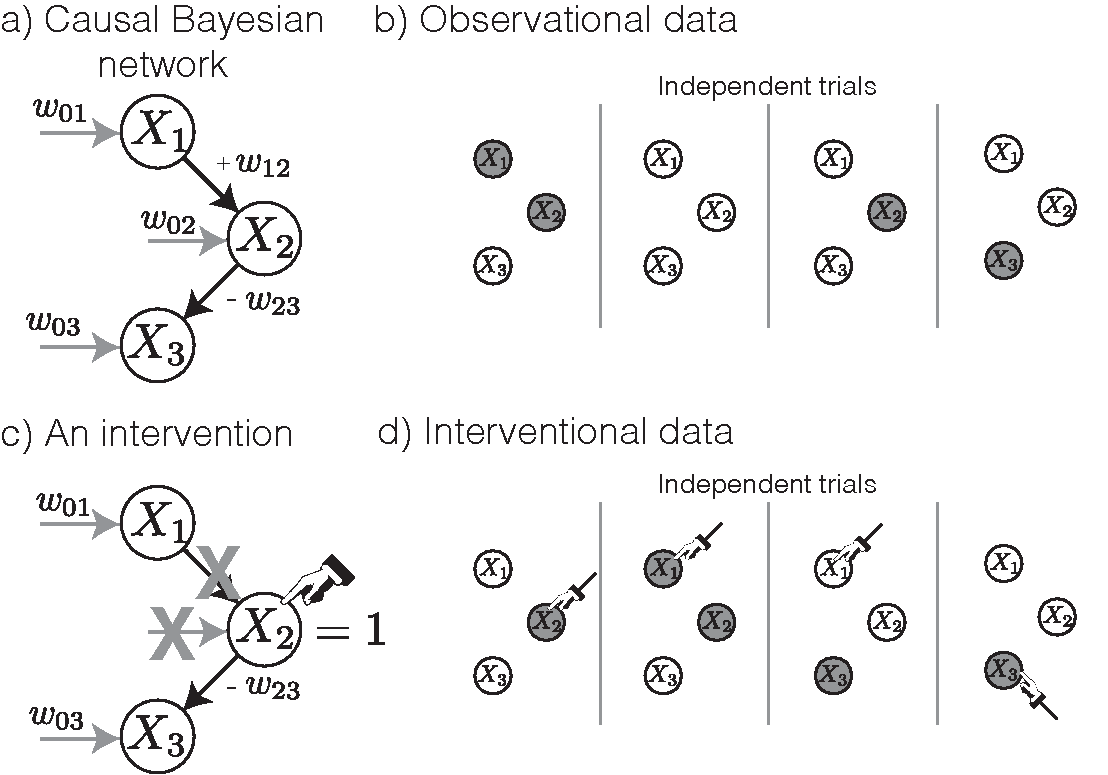
\includegraphics[width = .7\columnwidth]{CBNbw}
   \caption{a) A causal Bayesian network containing a generative connection (``+'' symbol) and a preventative connection (``-'' symbol) parametrised with base rates $w_{0i}$ and causal strengths $w_{ji}$.  b) Example observational data.  Shading indicates a variable was present (i.e., took the value 1) while white indicates a variable was absent (i.e., took the value 0) c) An intervention $\Do[X_2 = 1]$, disconnecting $X_2$ from $X_1$ and any background factors. d) Example interventional evidence.
   }
   \label{fig:CBN}
\end{figure}

\subsection{Modelling intervention choice}

Different interventions yield different outcomes, which in turn have different probabilities under different models.  This means that which interventions are valuable for identifying the true structure depends strongly on the hypothesis space and prior.  For instance fixing $X_2$ to 1 ($\Do[X_2\!=\!1]$) is (probabilistically) diagnostic if you are primarily unsure whether $X_2$ causes $X_3$ because $P(X_3|\Do[X_2\!=\!1])$ differs depending whether $X_2$ causes $X_3$.  However, it is not diagnostic if you are primarily unsure whether $X_1$ causes $X_2$ because $X_2$ will take the value 1 irrespective of its causes.  Optimal experimental design theory allows us to reason about the expected value of different interventions relative to a notion of uncertainty \citep{fedorov1972theory,raiffa1974applied}.  For instance, we can define the value of an intervention as the expected reduction in uncertainty about the true model after seeing what happened. This expectation can be calculated by averaging, prospectively, over the different possible outcomes of each potential intervention and computing the reduction in uncertainty in each case \citep[e.g.,][]{shannon1951prediction}. See \cite{bramley2017neurath} for a detailed mathematical account.

Well-chosen interventions can be much more informative about a causal system than mere observations.  The depicted observational data (Figure~\ref{fig:CBN}b) is much less informative than the interventional data (Figure~\ref{fig:CBN}d) with respect to the set $\mathcal{S}$ of all possible causal Bayesian networks relating the three variables.  
This is partly because the observational data does not distinguish between models with the same dependency structure, but also because a well-selected sequence of interventions can systematically target and resolve residual sources of uncertainty, for instance by testing a particular causal connection that previous tests have not provided clear evidence about.

\subsection{Causal Bayesian networks in psychology}

CBNs were initially adopted in psychology because of their ability to account for qualitative patterns of human judgments that are hard to capture under simple associative accounts of learning \citep[e.g.,][]{rescorla1972theory,holyoak2011causal,waldmann1992predictive,waldmann1998bayesian}.  
The idea that evidence is filtered through a causal model, provides a powerful account of human causal learning and reasoning \citep{cheng1997from,waldmann2000competition,griffiths2005structure}.  Several studies have also shown that people make structure judgments  from contingency information qualitatively in accordance with Bayesian network theory \citep{steyvers2009bayesian,mayrhofer2016sufficiency,rothe2018successful}.

Pearl's interventional ``Do'' calculus is an effective way of capturing the different ways in which people draw inferences based on observations or interventions \citep{sloman2005do,waldmann2005seeing}. While observations license backward inferences, interventions do not. Observing that your officemate arrives at the office soaked suggests that it may be raining outside, while if you had intervened and poured a bucket of water on them, their wet clothes would not tell you anything about the weather.  The notion that people can imagine virtual interventions helps explain important aspects of thinking.  For example, virtual interventions that ``try out'' different possible actions and play out their consequences are an important part of planning \citep{pfeiffer2013hippocampal,bramley2017phdthesis}.  Explanation often makes reference to counterfactuals \citep{lagnado2013causal,rips2013inference,rips2010two,lucas2015improved,gerstenberg2015how}, which are ``if statements'' referring to situations contrary to fact, such as: ``If Oswald did not shoot Kennedy, then someone else did''.  These kinds of inferences require a learner be able to imagine an intervention that makes the counterfactual true with minimal revision of the causal history \citep{gerstenberg2013back,rips2010two,lagnado2013causal}. 

The importance of interventional learning is well-established in education, and developmental psychology, where self-directed ``play'' is seen as vital to healthy development \citep[e.g.][]{piaget1930child, bruner1976play}.  Accordingly, a number of developmental psychologists have adopted a ``child as scientist'' analogy, which views children as fundamentally engaged in causal hypothesis testing within the CBN framework \citep{gopnik2000detecting,gopnik2004maps,sobel2006importance,mccormack2016children}.  In adults, a number of studies have found that people benefit from the ability to perform (or watch others perform) interventions during causal learning \citep{lagnado2002learning, lagnado2006time, lagnado2004advantage, schulz2001do, sobel2006importance}. 

Several recent studies have also explored \emph{how} people select what interventions to perform, comparing adults' and children's choices against the dictates of optimal intervention selection,  considering constrained and heuristic variants of this \citep{bramley2015fcs,bramley2017neurath,mccormack2016children,coenen2015strategies,steyvers2003intervention}.

\subsection{Shortcomings of CBNs for modelling everyday interventions}

In this section we highlight several mismatches between CBNs and the kinds of causal inference problems that characterize everyday causal cognition.  These break down into: 1. The requirement that evidence be gathered over independent trials; 2. the absence of temporal considerations relating interventions and subsequent measurements of the system; and 3. problems with representing cycles and feedback dynamics.

\subsubsection{Independent trials}

As we noted above, CBNs are very limited in their representation of time.  The interventional calculus embodies the minimal assumption that causes precede their effects, but it says nothing about the relative delays of competing causal pathways.  
Thus, CBNs are a natural partner to evidence that really has been gathered across multiple independent trials, in which causal relationships play out too fast to measure, or in which each variable is only measured once.  By design, these features are standard in real experimental data sets.  For instance, medical studies will typically involve a procedure for randomized recruitment to ensure participants are roughly independently sampled from the desired population. Then, there will be a protocol for when to measure outcome variables (such as blood pressure, insulin levels etc.) following an intervention (i.e., delivery of a treatment).  The use of a fixed trial protocol makes it straightforward to aggregate results across the sample.  However, choosing an appropriate schedule of treatment and measurement seems to require substantial preexisting causal expertise about how long the relevant mechanisms will take to work, and about when any effects will be most measurable.  

A consequence of the CBN framework being widely used to study causal cognition is that many of the experiments in the literature provide learning data that is already ``packaged'' into a CBN suitable format.  In early studies, participants were asked to make causal judgments based on data provided in tabular form detailing how often several variables appeared together or separately \citep{cheng1990probabilistic}.   In more recent studies, participants were shown a series of cases \citep{gopnik2000detecting,sobel2004children,deverett2012learning,lagnado2002learning},  or invited to choose a sequence of interventions of their own devising \citep{coenen2015strategies,bramley2015fcs,bramley2017neurath}.  But in these studies participants are instructed or given a cover story implying that each observation should be treated as a completely independent trial.   

In some cases, the cover stories involved artificial mechanisms that reset on each trial --- this includes the ``black box'' toys used in developmental studies \citep{mccormack2016children,gopnik2007causal,coenen2017beliefs}, but also a range of artificial mechanisms involving lights, sensors, circuits, and switches \citep{waldmann2000competition,sobel2006importance,coenen2017beliefs}.  In other cases, the nature of the variables is not described at all \citep{bramley2015fcs,bramley2017neurath,rehder2005feature}, or independence is established by instructing participants that each trial is performed with a different sample from a population \citep{rehder2003causal, rottman2012causal, rehder2017failures}.

While ingenious, these cover stories create situations that rarely obtain in everyday learning.  The causality we encounter in physical and social systems of everyday life do not, generally, reset themselves between each interaction \citep{greville2007influence,rottman2016searching}.  In life, one learning episode typically bleeds into the next, with no clear boundaries.  We might try a medicine on multiple occasions, but if we want to treat these tests as independent we had better leave a substantial amount of time between each test, relative to our beliefs about how long the drug takes to pass through our system.  We also must keep in mind the ongoing evolution of our health and potential adaptation in our receptivity to the medication. Choosing when to act, and how to delineate between and aggregate over ``trials'' in continuous experience \citep[cf][]{tulving1972episodic,gallistel2000time}, are important aspects of real world causal reasoning, that are missed by the studies focusing on CBN-packaged data.


\subsubsection{Timing of interventions and measurements}

In everyday life, observations cannot easily be separated \emph{between} trials, and learning from actions requires paying close attention to how things play out \emph{before, during} and \emph{after} interventions.   \cite{rottman2012causal} point out that it is often the \emph{change} in the state of a variable from one time point to another that people seek to explain.  Furthermore, it is hard to imagine intervening on something in the world without first observing its pre-interventional state.  The metaphysics of an intervention in a CBN not only presumes independence of one test from one another, but also imposes a practically implausible sequence of actions and measurements on the part of the learner.  An idealized intervention involves setting variables independently from the current states of the variables in the system, essentially \emph{before} observing their values \citep{pearl2000causality}.  Any causal effects of one's interventions are assumed to have entirely propagated through the system by the time the observation is made, while the trace of the resulting variable states must persist long enough to be measured together at the end.  
To make this work in psychology experiments, cover stories are used that are often either (i.) vague about the measurement of time, (ii.) pertain to variables whose states are only observable after the fact, or (iii.) involve causal relationships that would propagate too fast to be observed.  

\subsubsection{Cycles}

CBNs are based on a factorization of a joint probability distribution, meaning they cannot naturally represent relationships that form loops or cycles.  However, such dynamic relationships are pervasive in the world --- for example an increase in the abundance of a food source (e.g., grass) causes a population increase for animals that rely on that food source (e.g., locusts) that then reduce the abundance of the food source by eating it, which then causes most of them to die out, which again allows the food source to recover, and so on \citep{white2008beliefs,odum1959fundamentals}.  All sorts of real world processes, from population change \citep{malthus1888essay}, to economic, biological, and physical interactions, are characterized by reciprocal and dynamical causal processes giving rise to emergent behaviour like periodic oscillation, self regulation or self reinforcement.  In experiments, people frequently report causal beliefs that include cyclic relationships when allowed to do so (\citealp{nikolic2015there,kim2002clinical,sloman1998feature,rottman2014children}; but see also \citealp{white2008beliefs}).
While there are ways of adapting the CBN formalism to capture cycles (\citealp[e.g.][]{dean1989model,lauritzen2002chain}; and \citealp{rehder2016cycles} for a recent review) these either evoke a sequence of equally spaced discrete time steps or model the equilibrium behaviour of the system.  Thus, none of these proposals capture how cause--effect relationships unfold in continuous time, where some relationships might occur much faster or slower than others.

\subsection{Summary and discussion}

In sum, as we move away from carefully organized experimental scenarios toward more naturalistic interventional learning data, the assumptions that lend the CBN framework its mathematical simplicity also make it less adequate for the challenge.  
When we interact with the causal world, we typically have access to a lot more evidence than independent joint state measurements.  We can monitor variables continuously, tracking when events occur relative to one another and how continuous quantities ebb and flow over time.  We are sensitive not just to the ``final'' states of variables after causality has been and gone, but also to their states prior to interventions and their subsequent transitions.  To intervene effectively and to draw sensible causal conclusions by aggregating over extended experience, we must not only worry about what variables are relevant, but also when they should be measured, how much time to leave between tests, or how to best ``reset'' a system before testing it anew. 
This suggests that much of the important and interesting causal inference work in cognition takes place while packaging a learning problem into a CBN suitable format.  Independent trials are a luxury brought about through carefully curated scenarios, and aggregation to the level of contingencies and probabilities only becomes possible when we have rich enough knowledge of functional form to abstract away from time's arrow.  Thus, it is instructive to model this finer grain of human causal learning and reasoning in which time's arrow is fully represented.  
In the next sections, we build on these considerations and classic results about learning from temporal information, sketching two new approaches to modelling causal representation and interventional learning in continuous time.


%%%%%%%%%%%%%%%%%%%%%%%%%%%%%%%%%%%%%%%%%%%%%%%%%%%%%%%%%%%%%%%%%%%%%%%%%%%
\section{Incorporating time: Event data}\label{section:DN}
%%%%%%%%%%%%%%%%%%%%%%%%%%%%%%%%%%%%%%%%%%%%%%%%%%%%%%%%%%%%%%%%%%%%%%%%%%%

\subsection{Existing research}

People have been shown to make systematic use of both event order \citep{bramley2014order} and delay information in inferences about causal relationships \citep{buehner2003rethinking,buehner2004abolishing,buehner2006temporal}. Causal beliefs have also been shown to influence time perception \citep{bechlivanidis2013does,buehner2009causal,haggard2002voluntary}.  A basic associative learning result is that, as the average interval between two events increases, the strength with which these events are associated decreases \citep{wolfe1921effect,shanks1987associative, grice1948relation}.  However, people do not always see shorter intervals as more causal, but rather prefer intervals that match their expectations, where these might come from prior experience or through familiarity with causal mechanisms.  
Both shorter-than-expected and longer-than-expected intervals have been shown to reduce causal strength judgments \citep{buehner2004abolishing, schlottmann1999seeing,buehner2002knowledge,greville2010temporal,hagmayer2002temporal,buehner2003rethinking,greville2016temporal}.  Reliability also appears to be key to strong causal attributions from time, with variability in inter-event intervals normally associated with reduced causal judgments (\citealp{greville2010temporal,lagnado2010influence,greville2013structural}, although see \citealp{young2009problem}, for a counterexample).

Supporting the notion that temporal considerations inevitably feed into causal judgments, several studies have pitted temporal order cues against statistical contingencies.  These studies generally found that causal judgments were dominated by temporal information \citep{lagnado2006time,lagnado2004advantage,burns2009temporal,schlottmann1999seeing,frosch2012causal}.  For example,  \cite{lagnado2006time} explore a setting where a virus propagates through a network of computers infecting each with some probability, but also with variable delays in transmission from one computer to another. Participants' task was to infer the structure of these computer networks based on having observed viruses spreading through the network on multiple trials.  Participants preferred causal models that matched the experienced order in which computers displayed infection, even when covariational information (which subset of computers got the virus on each trial) suggested a different structure.  Furthermore, even when researchers have tried to instruct participants to ignore event timing, participants still often treated the observed timings of events to be diagnostic \citep{white2006structure,mccormack2016children}.  Additionally, a result common to several of the studies that have explored causal learning through interventions on CBNs, is that participants tend to draw direct connections from intervened-on components to their indirect effects \citep{bramley2015fcs, bramley2017neurath, mccormack2016children, fernbach2009causal}, ending with a kind of ``successor representation'' where each variable is associated with all of its proximal and distal consequences \citep{dayan1993improving,momennejad2017successor}. This suggests that people find it unnatural for events to cause one another when they seem to occur at the same time. 

\subsection{Representing causal events and interventions in time}


\begin{figure}[h!]
   \centering
   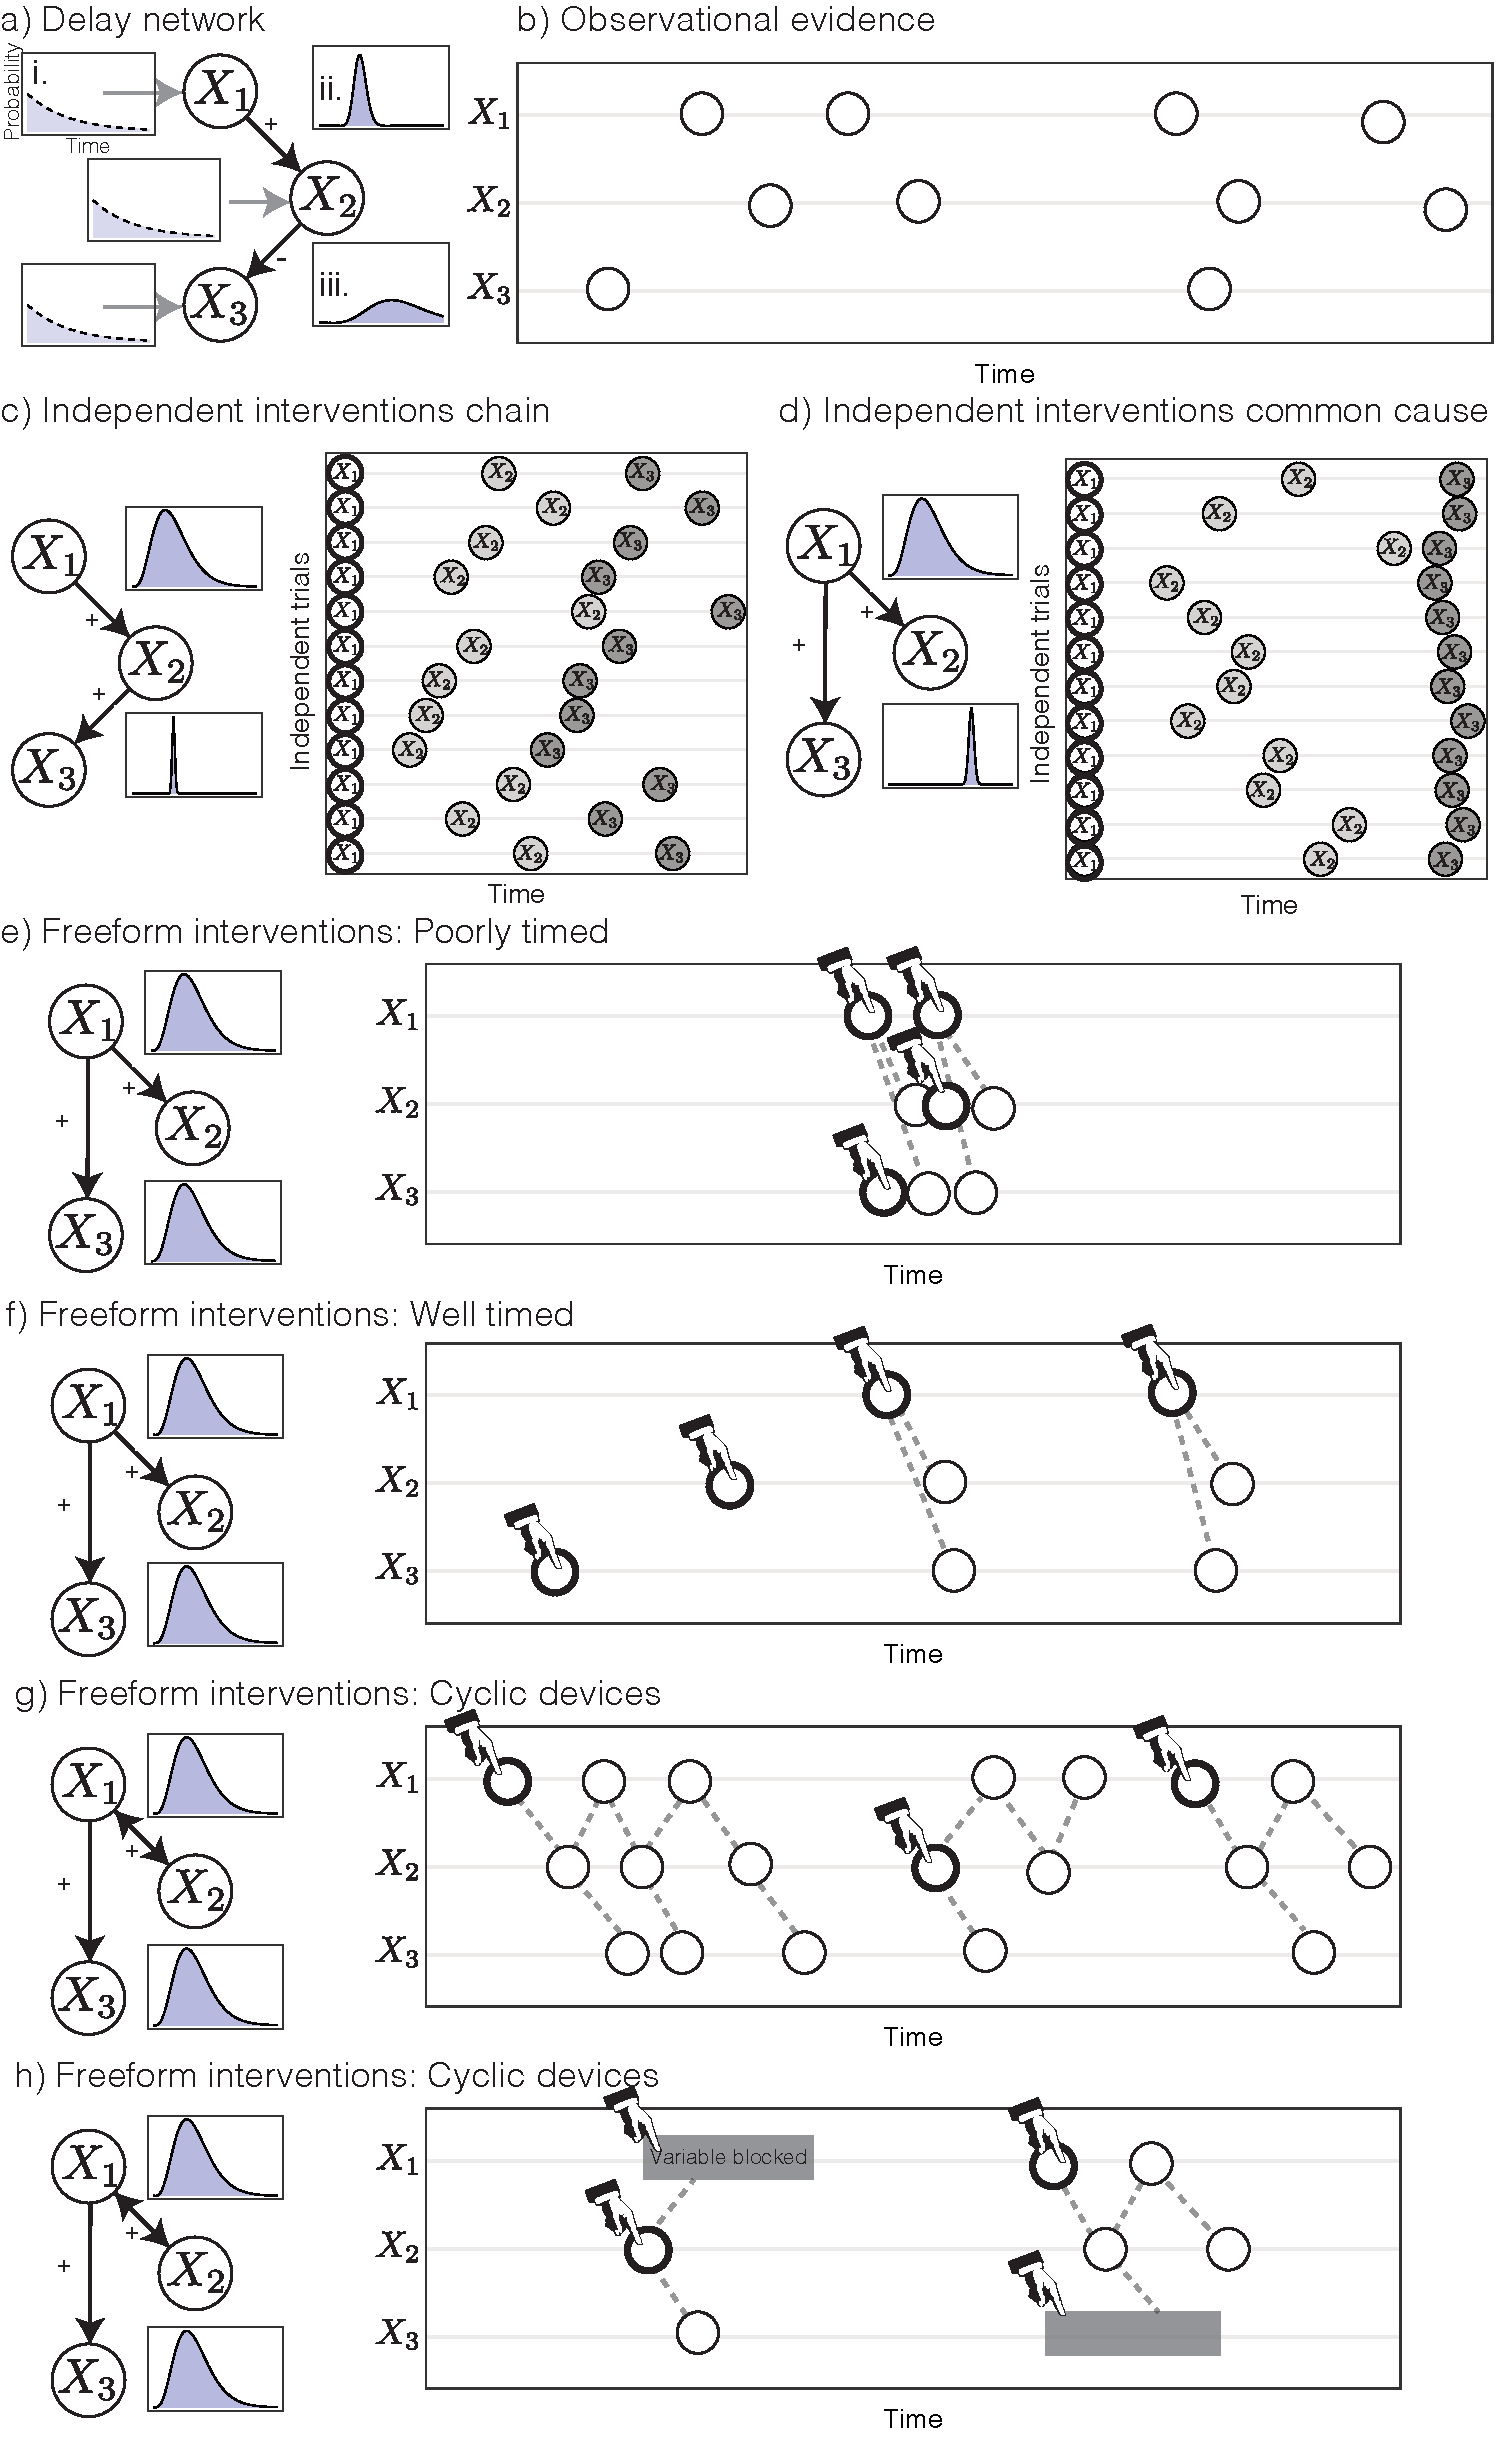
\includegraphics[width = .78\columnwidth]{DN}
   \caption{\scriptsize{a) Example causal delay network showing interevent delay densities for constant base rate (i.), and following a generative (ii.) or preventative (iii.) cause.  Rows denote variables and white circles mark activations over time.  c) Independent interventions on $X_1$ (rows) in a chain structure. d) Independent interventions on a common cause structure.  
   e) Example freeform interventions that are not well spaced.   Rows denote variables, hand symbols and thick borders denote interventions, circles denote activations.  Dashed grey lines show the actual causal influences.  f) As in e) but interventions more widely spaced.  g) Interventions in a cyclic network. h) Including ``blocking'' interventions that temporarily prevent activations of the blocked variable and so break feedback loops.}}
   \label{fig:DN}
\end{figure}

To account for time sensitivity in structure induction over multiple variables, we need a causal representation rich enough to encode beliefs about causal inter-event delays.  
\cite{bramley2018time} recently developed a normative framework that does this. 
Concretely, our framework captures causality between events (hereafter ``activations'') that occur at components of a system $X_1,\ldots,X_n$ at particular points in time, but have no measurable duration of their own \citep{cox1980point}.  \citeapos{bramley2018time} approach captures activation patterns within a causal system as being produced by a mixture of exogenous influences and endogenous causal relationships, with parametric delays governed by Gamma distributions with some mean $\mu$ and shape $\alpha$. Figure~\ref{fig:DN}a gives an example of an  $X_1\!\stackrel{+}\rightarrow\!X_2\!\stackrel{-}\rightarrow\!X_3$ chain analogous to the CBN in Figure~\ref{fig:CBN}.  
As in a CBN we can assume all three variables are activated due to exogenous factors with their own ``base rate'' probability.  This can be captured by a Gamma distribution where shape $\alpha$ is set to 1, equivalent to an Exponential distribution.  This means that the expected delay before the next activation of $X_1$ is constant, regardless how long it has been since the last activation of $X_1$ or any other variable.  Activations of $X_1$ then cause activations of $X_2$ with a short and somewhat variable delay (see Subfigure~\ref{fig:DN}a, ii).  These caused activations are in addition to any activations of $X_2$ caused by its base rate.  Thus, the model implies that we should expect to see $X_2$ activate shortly after observing $X_1$ activating.  Activations of $X_2$ then have a preventative effect on $X_3$.  This is modelled by having activations of $X_2$ block the subsequent activation of $X_3$.  Mathematically, this changes the distribution for $X_3$ from an Exponential back to a Gamma, doubling the time we expect to wait until seeing $X_3$ again but also introducing a temporary dependence between latest $X_2$ and the next $X_3$ (see Subfigure~\ref{fig:DN}a, iii).  \cite{bramley2018time} provide the mathematical details for estimating model parameters and incorporating base rates and failure rates (similar to causal strengths in CBNs), as well as modelling conjunctive or disjunctive combined causal influences. However, here we simply highlight what we learn about causal cognition by applying this framework to human judgment and intervention patterns.  

\subsection{Modelling inference}

Unlike the CBN case, \citeapos{bramley2018time} approach captures how timing information informs structure judgments across potentially open-ended learning periods, without the necessity of independent trials.  If a learner already has a strong domain prior, for instance that a particular causal relationship will take a certain length of time to work, this will drive their judgments from temporal information in a straightforward way.  That is, they will only think an event caused an outcome if the interval between cause and effect matches their expectation.  However, different structures map inter-event intervals to different cause-effect delays, meaning that even without specific prior expectations about delays, the ability of candidate structures to parsimoniously account for the data can be compared, analogous to fitting a CBN to contingencies without a prior knowledge of the plausible parameters.  If a learner starts out with no expectations about how long or how reliable causal delays will be, Bayesian Ockham's razor will still favour whatever structure can assign the highest likelihood to the patterns of time dependence observed between variables, while requiring the fewest separate delay parameters \citep{bramley2018time}.   For example, the reliable $X_1-X_2$ intervals in Figure~\ref{fig:DN}b will favour models that include a generative $X_1\!\stackrel{+}\rightarrow\!X_2$ connection since this can explain the activations of $X_2$ better than a model presuming them to be exponentially distributed or to be caused by any of the other variables.

\cite{bramley2018time} show that people spontaneously make structure judgments from event data, broadly in line with the normative framework described above.  In three experiments, participants were asked to judge which of a range possible causal structures best describe the activations of components of a set of causal devices.    In one experiment, participants were presented with four video clips of each causal device, each showing all of the devices' components activate over 3-4 seconds.  Each video begins with the activation of the root component ($X_1$) followed by the activation of three other output components ($X_2$ and $X_3$ and $X_4$) in varying orders with varying intervals.  Participants not only ruled out structures that could not have produced all of the observed patterns, but also assigned more probability to structures to the extent that could have reliably produced the observed delay patterns.

While \cite{bramley2018time} modelled the induction of general causal structure knowledge (e.g., learning that $X_1$ causes $X_2$), \cite{stephan2018latency} have adopted the framework and proposed a model of causal attribution explaining how reasoners apply their knowledge about causal delay distributions to answer causal queries about singular cases (e.g., did $X_1$ cause $X_2$ on a particular occasion for which it is known that $X_1 = 1$ and $X_2 = 1$). In particular, \cite{stephan2018latency}  showed that causal delay information must be considered to account for the possibility of causal preemption of a target cause (e.g, $X_1$) by an alternative cause (e.g, $X_3$).  That is, the possibility that even though $X_1$ was on its way to causing $X_2$, some other background cause $X_3$ might have ``gotten in first'' and already caused $X_2$. This is a problem that singular causation judgments are highly sensitive to, but that cannot be handled by preexisting accounts of causal attribution.

\subsection{Modelling interventions}

Just as with covariational observational data in Figure~\ref{fig:CBN}b, pure observations of events in time cannot unambiguously reveal causal structure.  For example, it could be the case that the tight temporal relationship between $X_1$ and $X_2$ in Figure~\ref{fig:DN}b comes about because the variables share an unmeasured cause that brings about $X_1$ faster than it brings about $X_2$.  Fortunately, intervention again makes it possible to resolve these kinds of ambiguity.  Any temporal dependence between the intervened-on variable and activations of other variables suggests the presence of a causal influence.  For this to hold, interventions must be performed at random or prechosen intervals so as to be temporally independent of any alternative causes.  Concretely, for two variables $X_i$ and $X_j$, if the distribution of inter-event delays $p(t_{X_j, X_i})$ has a best-fitting $\alpha$ parameter $>1$, this means that $X_j$ hastens $X_i$ relative to its baseline, implying that $X_j$ (directly or indirectly) influences $X_i$.  
A key property of \citeapos{bramley2018time} modelling framework is that it captures how the sequence of events following an intervention carries information about the underlying causal structure. Post-interventional event \emph{order} places constraints on what caused what on a given occasion.  But beyond this, the causal delays inherit time variability from their parents relative to interventions.  Thus, even if an intervention causes the same activations in the same order each time, if the timing of one of these downstream events carries information about another later one, this tells us something about the causal ordering of the variables.  Figures~\ref{fig:DN}c and d visualize evidence produced by interventions on the root component of a chain and a common cause device.   The device in Figure~\ref{fig:DN}c is in fact a chain where $X_1\!\stackrel{+}\rightarrow\!X_2\!\stackrel{+}\rightarrow\!X_2$ with two fast connections, one unreliable connection from $X_1\!\stackrel{+}\rightarrow\!X_2$ and another reliable connection $X_2\!\stackrel{+}\rightarrow\!X_3$.  This is revealed by the data for the chain structure: if $X_2$ happens late, $X_3$ tends to happen late as well.  However below we see a $X_3\!\stackrel{+}\leftarrow\!X_1\!\stackrel{+}\rightarrow\!X_2$ with one unreliable fast connection $X_1\!\stackrel{+}\rightarrow\!X_2$ and one reliable slow one $X_1\!\stackrel{+}\rightarrow\!X_3$.  Here the $X_1\!\stackrel{+}\rightarrow\!X_2$ and the $X_1\!\stackrel{+}\rightarrow\!X_2$ delays are uncorrelated.  

We can think of the propagation of variability through the system as acting akin to a game of ``broken telephone''.  In broken telephone, players form a line and then whisper a message from one person to the next, becoming increasingly garbled along the way.  Knowing what message a player heard tells you roughly where in the line of people they were.  Similarly, the accumulation of errors in a signal (here in the lateness or earliness of the event timing) can reveal the causal sequence.  As with broken telephone, if there is no noise (if everyone passes the message perfectly; or if all causal relationships are perfectly reliable) there is no way to tell in what order the message was passed on. But, a moderate amount of noise can lead to a ``blessing of variability'' effect.\footnote{The same thing holds for covariational data under certain parametrisations.  For example with no background noise and weak causal connections the latter links in a chain become progressively less likely to be present.}   \cite{bramley2018time} show that people are sensitive to this subtle signal, favouring chain structures for a range of scenarios in which a mediating variable carries information about a distal effect $X_3$ and common cause structures when it does not.  

\subsection{Choosing when and where to intervene}

\citeapos{bramley2018time} approach is applicable to situations where variables may activate or be intervened on multiple times during a single learning period, and in which the underlying structure might contain cycles.  Thus, \cite{bramley2017dynamic} also used the framework to explore learners' choices of interventions in extended interactions with unknown causal systems.  Instead of giving participants a sequence of independent trials in which to set variables as in traditional interventional learning studies, participants were given a short time to interact with a dynamic causal system and perform a small number of interventions by clicking on components on the computer screen to activate them.\footnote{See \url{https://neilrbramley.com/experiments/it/videos/example\_trial.html} for a video of a trial.}   In this setting, learners had to choose both when and where to intervene.  \cite{bramley2017dynamic} explored learning about a mixture of acyclic structure (no feedback loops) and cyclic structures (containing at least one feedback loop), and contrasted learning about devices whose causal delays were known to be reliable (1.5 seconds with standard deviation 0.1 seconds) with those that were known to be unreliable (1.5 seconds with standard deviation 0.7 seconds) .  Causal connections had a small failure rate and there were no exogenous activations aside from the learners' own interventions.  Consistent with the predictions of the normative model sketched above, \cite{bramley2017dynamic} found that participants were able to identify the majority of the causal connections based on the delayed activation information they produced, and were more accurate at identifying the structure of the devices when the delays were reliable. 

\cite{bramley2017dynamic} found that successful participants tended to leave large and regular intervals between each intervention, especially when the true causal relationships were unreliable.  Successful participants also tended to wait longer after the most recent activation before intervening again, suggesting they waited until they had a low expectation that any other confounding activity would occur during their intervention.  For example, Figure ~\ref{fig:DN}e shows a poorly chosen set of interventions that occur close together, making it ambiguous which activations caused which.  By contrast, the well-spaced interventions in Figure ~\ref{fig:DN}f make it clear that $X_1$ is a common cause of $X_2$ and $X_3$.  Both $X_2$ and $X_3$ reliably follow from the two interventions at $X_1$ but, on the second occasion, $X_2$ and $X_3$ reverse their order of activation, essentially ruling out the $X_1\!\stackrel{+}\rightarrow\!X_2\!\stackrel{+}\rightarrow\!X_3$ chain hypothesis that was a plausible up to that point.  No study has explored preventative causation in the domain of continuous time causal events. However, by contra-position to the above, the ideal time to test for a preventative relationship (as in the $X_2\!\stackrel{-}\rightarrow\!X_3$ link in Figure~\ref{fig:DN}a) should be when one has a strong expectation the effect is otherwise about to occur.  

For the acyclic devices tested in \cite{bramley2017dynamic}, participants exhibited a substantial preference for intervening on the root components, an effect also found in CBN-based studies \citep[e.g.,][]{coenen2015strategies, bramley2015fcs}.  Unlike in most CBN-based experimental settings, these positive test interventions \emph{are} informative about the relationships between the downstream variables due to the blessing of (moderate) variability described above.   By intervening at the root of the causal device, learners can  observe how the causality propagated through the system making use of ordering and delay correlations to uncover the causal sequencing. Thus, it could be that positive testing effects are largely a result of the overapplication of a strategy that works well in the real world where we can normally expect to experience the effects of interventions playing out over time.

\citeapos{bramley2017dynamic} experiment is also the first comparison of human learning about acyclic and cyclic devices in continuous time.  Participants' interventions on cyclic devices often led to sustained patterns of activation that continued until a failed connection caused the system to acquiesce.  This meant that participants experienced substantially more events in total even though they tended, reactively, to perform substantially fewer interventions on the cyclic devices.  While this resulted in stronger evidence about structure for the cyclic problems according to the normative learning model, the data was also much more computationally taxing to deal with in real time given the variability in the true causal delays.  The pattern in Figure~\ref{fig:DN}g demonstrates this.  It is clear from the repeated activations that $X_1$, $X_2$ and $X_3$ are related in some cyclic way.   However, establishing the exact set of connections (i.e., whether $X_2$ or $X_3$ feeds back to $X_1$) is much harder. There are also many plausible patterns of actual causation that could have given rise to this data --- that is, there are many ways one could draw dashed lines as in the figure, to attribute each activation uniquely to a unique previous activation or intervention.   To estimate the posterior probability distribution over potential structures, the model needs to sum over large numbers of patterns of possible actual causation \citep{halpern2016causality}.  Thus, it is not surprising that human learners with limited cognitive resources, were substantially worse at identifying the structure of the cyclic devices.  \cite{bramley2017dynamic} account for this result by positing that human learners build up their causal models incrementally, reacting to each new activation by attributing it to a recent intervention or activation.  When there are many causal influences going on simultaneously, this approach becomes less accurate.

\subsection{Summary and discussion}

We have developed a normative framework for representing causal structure relating events that unfold in time, and used it to explore real time causal learning and intervention selection.   Applying this framework to experimental data demonstrated that people use temporal delays between events systematically to infer the causal structure that most parsimoniously explains what happened.  %
The framework also showed that people are able to choose sensibly \emph{when} to intervene, so as to not confound the consequences of their interventions with the unfolding dynamics of the system. The framework captured why people have a preference toward initiating the root component of causal systems --- unlike the CBN-packaged data, this more natural temporally extended data often contains evidential signals about the structure of causality as action propagates though the system.

The analyses also shed light on the intuition that cyclic systems are naturally harder to learn and reason about. The computational cost of exact inference in \citeapos{bramley2018time} framework increased with the number of events that might be related, and cyclic systems tended to produce more activations and noncausal regularities.  The interventions investigated by \cite{bramley2017dynamic} can be thought of as ``shocks'' to the system, where an additional event is injected into the system by the learner.  One way that learners might get clear evidence about dynamic systems in real world contexts is by using extended interventions to ``block'' rather than just ``shock'' variables. By ``blocking'' we mean holding a variable in a particular state for an extended period, while ``shocking'' instantaneously changes the value of a variable but does not hold it in that position.  In the current punctate event context, a blocking intervention could be to prevent a variable from activation thus disconnecting it from participating in the causal process.\footnote{In continuous variable contexts like the one discussed in the next section, ``blocking'' has a different interpretation: namely holding a variable at a particular value for an extended period.}  Figure~\ref{fig:DN}h considers a case in which a hypothetical learner uses a mixture of interventions similar to above, with extended ``block'' interventions that prevent the blocked variable from activating for a period of time.  This ``blocking'' action is analogous to setting a variable to 0 in the CBN setting explored in \ref{section:CBN}. Blocking breaks the feedback in the system allowing the learner to identify one part of the structure at a time as they would in the acyclic cases.  As we discuss at the end of the chapter, future work could explore how people use a combination of ``shocks'' and ``blocks'' to learn about cyclic systems.

\cite{lagnado2004advantage} proposed that real-time interventions exhibit a strong order cue: events that happen shortly after interventions are likely to have been caused by these interventions.  \citeapos{bramley2018time} framework captures under what conditions this heuristic works well, but also formalizes how interventions provide structure evidence regardless of whether this holds.  If the base rates of variable activations are low relative to the duration of actual causal delays, interventions that activate the cause will tend to create a reliable order cue.  That is, effects of the intervention will frequently be the next activations to occur as they are in Figure~\ref{section:DN}e.  The fact that participants struggled when there was a dense flurry of activations in \cite{bramley2017dynamic} is suggestive that people really do rely on this kind of cue to build up their hypotheses.  
However, the normative framework also captures how inference is possible even when this does not hold.  Wherever interventions on one variable affect the distribution of delays between that variable and another, either hastening or delaying them relative to their baseline, this is evidence for some form of causation.

Unlike with a CBN, a learner who forms a time-extensive representation is also positioned to make real-time predictions about ongoing dynamics \citep{clark2013whatever}.  This allows them to allow for ongoing causal processes in choosing when to intervene.   This was evident in \citeapos{bramley2017dynamic} experiment in which successful participants waited for activity to die out before intervening again.

One weakness of \citeapos{bramley2018time} approach is that normative inference scales rapidly with the density of events experienced relative to the length of the causal delays, meaning that cyclic or multiply connected structures become very hard to evaluate.  One has to reason about many potential paths of actual causation playing out simultaneously.  Fortunately, as the number of potentially related events becomes unmanageable for reasoning at the level of one-to-one cause-effect mappings, one can start to reason at a slightly rougher grain, about whether activations and interventions affect the \emph{rates} of occurrence of other variables.  \cite{pacer2015upsetting} model this setting, reanalysing an experiment from \cite{lagnado2010influence} in which the occurrence of several types of ``seismic waves'' could temporarily alter the rate at which earthquakes occur.  This approach matches with a range of findings suggesting that beyond a small number of unique entities, people switch to approximate counting, known as ``subitising'', rather than attempting to focus explicitly on each individual entity \citep{mandler1982subitizing}.

Another limitation of \citeapos{bramley2018time} approach is its assumption that causality relates to point events.  This idealization seems reasonable for processes where the causal influences are occasional and sudden --- such as spiking neurons, earthquakes, gunshots, explosions and so on.  However, many other causal influences are continuous in time, and many causally relevant variables can take a continua of values with no transition or state being causally privileged.  Thus, in the next section we extend the continuous time framework to capture learning and inference about variables that evolve and affect one another continuously in time.

%%%%%%%%%%%%%%%%%%%%%%%%%%%%%%%%%%%%%%%%%%%%%%%%%%%%%%%%%%%%%%%%%%%%%%%%%%
\section{Incorporating time: Continuous variables}\label{section:ctcv}
%%%%%%%%%%%%%%%%%%%%%%%%%%%%%%%%%%%%%%%%%%%%%%%%%%%%%%%%%%%%%%%%%%%%%%%%%%


While events are often a natural level for reasoning about the world, they need not be construed as discrete or punctate, and change need not be thought of as being constituted by \emph{events} at all \citep{soo2018causal}.  Many variables change continuously over time without clear change points, and their consequences can often ``linger on and mix with the effects of other actions'' \citep[p224]{jordan1992forward}. This means that in many contexts, better causal evidence can be had, and finer grained causal predictions can be made, if one represents the causal world as a system of continually interacting continuous-valued variables.  Many real-world applications of causal inference methods focus on this kind of data.  Financial forecasting, climate research, and many aspects of structure estimation in neuroscience involve reasoning about causal influences between continuous variables.   The most well-established of these approaches is the so called ``Granger causality'', which uses time-delayed regressions to assess whether one variable predicts the later values of another \citep{granger1969investigating}.  \cite{soo2014learning} show that such change-time asymmetries are an important determinant of human causal judgments.  However, this approach suffers from the same limitations as any observational method for assessing causality.\footnote{Although, see \cite{eichler2010granger} for preliminary work linking interventions with estimates of Granger causality.}  Frequently variables \emph{Granger cause} one another without truly causing one another, due to their both being influenced by some unmeasured common cause.  For example, because neural activity waxes and wanes due to natural circadian rhythms, regressing one neural signal on another, even with a short delay, will often result in a significant correlation because both measurements share patterns of variation that stem from the brain's overall energy consumption rather than from specifically directed communication.    
A number of studies have also explored how people learn continuous valued functional relationships more generally, but not in the context of inferring causal structure \citep{pacer2011rational, griffiths2009modeling, schulz2017compositional}.  So, in this last section, we survey a framework for modelling interventional causal learning about continuous valued variables that influence one another in continuous time. Note we are not arguing this framework supersedes that of \cite{bramley2018time}, but rather that it is able to capture another form of time sensitivity that is appropriate for some learning contexts but inappropriate for others.

\subsection{Representing continuous causality}

\begin{figure}[t]
   \centering
   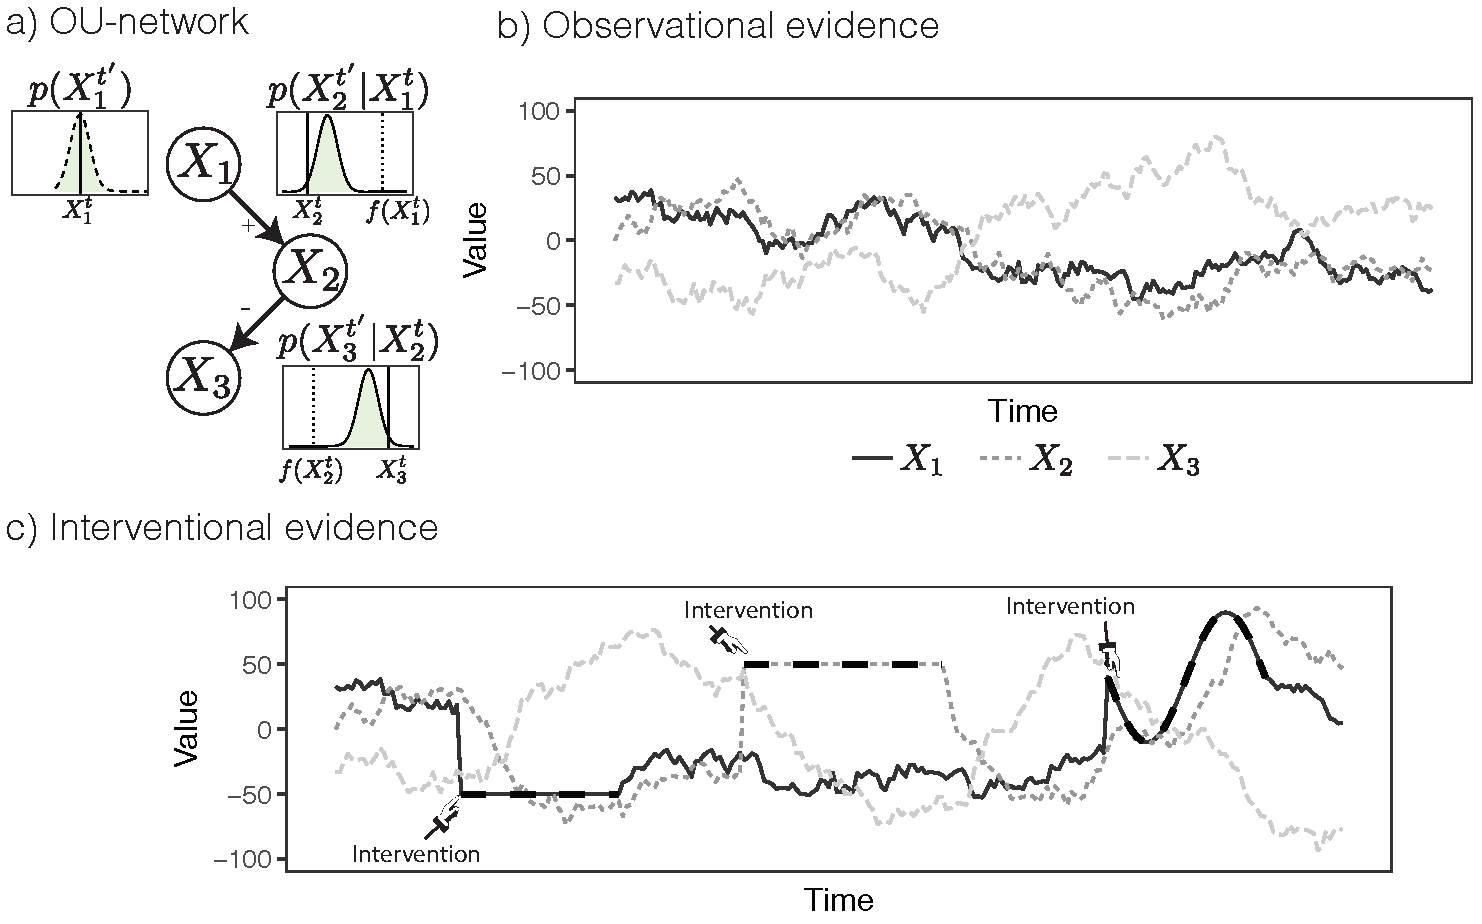
\includegraphics[width = \columnwidth]{OU_bw}
   \caption{Observations and interventions on a causal chain relating continuous variables in an Ornstein-Uhlenbeck network, adapted from \cite{davis2018ctcv}.    a) Visualisation of network and transition probabilities between $t$ and $t^{\prime}$ relative to states latest states of effect $X_j$ and cause $X_i$. b) Observational evidence in which OU-network from a is simulated forward.  Solid  black line = $X_1$, green dotted dark grey line $X_2$, dashed light grey line = $X_3$. c) Example of interventional evidence.  Heavy black dashed lines indicate interventions that hold variables in position or move them systematically.}
   \label{fig:OU}
\end{figure}

\cite{davis2018ctcv} recently developed a new framework for modelling networks of continuous valued variables interacting causally with one another.  Their approach is based on the Ornstein-Uhlenbeck (OU) process \citep{uhlenbeck1930theory}.  
OU processes describe something like Brownian motion that is subject to a corrective force that increases the further the variable strays from its mean and  
have been used to model a variety of phenomena including physical \citep{lacko2012planning} and financial \citep{barndorff2001non} systems as well as attention during multiple object tracking \citep{vul2009explaining}.  \citeapos{davis2018ctcv} insight was to treat all the relationships in a causal network as simultaneously evolving OU processes, such that each variable is noisily attracted to some function of the current states of its cause(s).    
To model ongoing causal relationships, the mean attraction state for a variable $X_i\in\mathcal{X}$ is defined as some function of the latest value of its putative cause variable(s) $X^t_j$.\footnote{Here we express OU dynamics between small but discrete equal time steps.  However, in its general form an OU process is described by a stochastic differential equation, making it truly continuous over time.}  \cite{davis2018ctcv} focus on linear relationships, with a single multiplicative parameter $w_{ji}$, such that the updated value of $X_i^{t^{\prime}}$ is given by

\begin{equation} \label{cont_OU_def}
X_i^{t'} = X_i^{t} + N(\theta\big(\sum_{j=1}^{\mathrm{ca}(i)}w_{ji} \cdot X_j^t - X_i^t\big),\sigma)
\end{equation}
where $\sigma$ is the noise level and $\theta$ controls how strongly the cause(s) influence the effect.  
Thus, if $w_{ji}>0$, $X_i$ will be attracted to some positive fraction of the value of the latest value of $X_j$ if it has just one cause, where this is assumed to be the sum over all causes $j\in\mathrm{c}(X_i)$ if there is more than one.  In line with the previous sections, we call this a ``generative'' connection as it implies that increases in $X_j$ cause increases in $X_i$.  If $w_{ji}<0$, $X_i$ will be attracted to some negative fraction of the latest value of $X_j$, with $X_i$ tending to decrease as $X_j$ increases and visa versa.  Values of $w_{ji}$ between $-1$ and $1$ will make $X_i$ undershoot the absolute value of $X_j$, while values greater than 1 or less than -1 will make $X_i$ overshoot. There is no causal relationship from $X_i$ to $X_j$ if 
the attraction strength $\theta_{ji}=0$.  If a variable has no causes, its movement can be modelled as a classical random walk or as tending revert toward some static mean value.  
\cite{davis2018ctcv} assume multiple causal influences sum in determining the attractor state for the effect.  
Figure~\ref{fig:OU}a shows an example continuous variable network $X_1\!\stackrel{+}\rightarrow\!X_2\!\stackrel{-}\rightarrow\!X_3$ analogous to those explored in Sections~\ref{section:CBN} and \ref{section:DN}.  In it, $X_1$ has no causes.  $X_1$ is then a generative cause of $X_2$ 
which is a preventative cause of $X_3$. 
The subplots visualize the distribution of possible $X_i^{\prime}$ values for each variable relative to the variable's current position and the current position of its cause.

Figure~\ref{fig:OU}b shows example data generated by the network in Figure~\ref{fig:OU}a.  The root component $X_1$ (red) drifts around randomly, while $X_2$ (green) chases noisily behind $X_1$, and $X_3$ (blue) chases the inverse of $X_2$.  As with previous settings, it is not possible to tell for certain what the right causal relationships are, based on this purely observational data.  This is partly because all three variables could be effects of some common cause with different time lags (i.e., with different $\theta$ values). Additionally though, the sustained corrective causal influences mean the downstream variables $X_2$ and $X_3$ rapidly asymptote to be close to their target values, making it hard to see which moved first unless $X_1$ happens to move dramatically.  

One interesting property about these continuous time networks that is not captured by the event networks in Section~\ref{section:DN} is their ability to produce rich emergent feedback dynamics of the kinds observed in the natural world.  
For example a pair of variables with bidirectional influences that undershoot one another (i.e., $w_{ji}=w_{ij}<1$) creates an inhibitory feedback loop where both variables trend toward and then stay around zero no matter their starting point, while settings where the feedback leads to progressively larger overshooting (i.e., $w_{ji}=w_{ij}>1$), excitatory feedback, where the variables rapidly approach positive or negative infinity.  
Feedback with opposite signs (i.e., $w_{ji} = -w_{ij}$) leads to oscillations such as those seen in predator--prey dynamics, where variables chase one another up and down in oscillations that can either acquiesce or can increase in magnitude over time.  Since these kinds of emergent dynamics are common in the natural world, it is valuable to have a simple representation that is able to mimic them.  However, it remains to be seen how commonly observation of high level dynamics uniquely reveals the internal structure of the system, as it may be that there are multiple ways of setting up a system of variables to exhibit the same emergent behaviour.


\subsection{Modelling inference and interventions}

\cite{davis2018ctcv} devised a simple experiment to explore human interventional learning about continuous valued variables in continuous time.  As in the studies discussed in Sections~\ref{section:CBN} and \ref{section:DN}, participants were tasked with identifying the structure of a number of causal devices by interacting with them on the computer screen.  As in \cite{bramley2017dynamic} they were given a short period to interact with each device.  However, rather than being visualized as clickable nodes, the variables were visualized with vertical sliders.  The underlying network could contain generative $w=1$ and preventative $w=-1$ connections and feedback loops.  Unless intervened on, the sliders' positions updated continually, 
appearing to jitter and track up and down as in Figure~\ref{fig:DN}b. By intervening and moving the sliders, participants could hold variables at desired values or drag them up and down.
\footnote{See \url{https://neilrbramley.com/experiments/ctcv/demo.html} to try an example trial.}

Through interacting with the systems, participants were able to identify the large majority of the connections.  As in the other causal learning experiments discussed, the most frequent error was a failure to distinguish direct and indirect causal influences.  Participants would often mark direct connections from intervened on variables to indirect effects.  Due to the convenient mathematical properties of OU processes, Bayesian inference could again be used to estimate a posterior for each trial and used as a normative standard against which to compare participants' judgments.  \cite{davis2018ctcv} compared full Bayesian inference against a local computations model that assumed learners built up their models by focusing on one pair of variables at a time rather than the whole structure, finding that around two thirds of participants were better described by this heuristic \citep[cf][]{fernbach2009causal}.  The normative analysis also revealed that with only one exception, participants interventions dramatically increased the strength of the available evidence.

The role of interventions in this continuous context intuitively has an additional property compared to the previous contexts.  Because the variables are capable of taking a wide range of values but naturally move only a little per timestep, interventions allow learners to inject dramatic swings and signals into the system, or hold variables at extreme or unusual levels \citep[Figure~\ref{fig:OU},][]{davis2018ctcv}.  For example, Figure~\ref{fig:OU}c shows a learner performing several dramatic interventions.  First they intervene to hold $X_1$ at 50 (here, for 40 ``timesteps'').  This results in a marked increase in $X_2$ and, with more noise and lag, a reduction in $X_3$.  They then intervene to hold $X_2$ at -50 which only increases $X_3$, while $X_1$ returns to moving randomly, suggesting the structure is a chain.  Third, they intervene on $X_3$ in a sinusoidal pattern leads to a (lagged and noisy) sinusoidal pattern in $X_2$.  While \cite{davis2018ctcv} did not analyse participants precise intervention patterns, a large proportion appeared to involve moving and holding variables at extreme values, or rapidly dragging them up and down the full range of the sliders.  It is worth noting that in this setting, interventions naturally act as both ``shocks'' and ``blocks''.  Intervening on a variable for an extended period not only takes over its state but also blocks it from participating in feedback dynamics.

\subsection{Continuous time control}

The interventions participants could perform in \cite{davis2018control} were often extended in time, meaning participants were able to react to the movements of the other variables during their intervention, for example they might be manipulating one variable in such a way as to keep another (effect) variable in a particular position.  
This reactivity brings the interventional learning problem increasingly close to an adaptive or ``dual control'' problem \citep{feldbaum1961dual,guez2015phd,klenske2016dual,schulz2017control}. This means one faces the ``dual'' problem of learning how the system works while already attempting to control it. For example, we learn to play tennis, largely, while attempting to play tennis. At first our shots are wild and do not go where we intend. But, we slowly learn to adapt our swing to different angles and speeds of the incoming ball hopefully building a causal control model of tennis in the process.

A key question therefore, is to what extent people will spontaneously learn causal structure while attempting to master the control of a causal system.  To investigate this, \cite{davis2018control} used their OU driven causal models as a class of control problems.   Their task was similar to that in \cite{davis2018ctcv}, except that participants' interventions were restricted to one ``control'' variable, and limited single step increments up or down.  Participants' goal was to keep another ``target'' variable in a reward region.  To master this task in a model-based way, a participant would have to learn the structure of the network and use this knowledge to plan the actions that maximize the time that the target variable stays in the reward region.  
Overall, participants learned to control all in most causal systems well above chance, and learning profiles were broadly consistent with the idea that they first explored then exploited the causal model.  Future work will need to carefully probe what representation participants for during a control period.


\subsection{Summary and discussion}

In summary, networks made up of OU-related continuous variables provide a powerful extension of causal models for reasoning about fine-grained continuous time relationships, as well as providing an interesting test bed of control environments.  The dynamics of these systems map onto real world problems in intuitive ways and display the kinds of emergent properties we see in real world dynamic causal systems.  These networks also have convenient mathematical properties that make normative inference tractable and so allow assessment of the evidential value of interventions.  OU processes are unique in being Gaussian, Markovian, and stationary, all of which make likelihood estimation closed form and straightforward \citep{uhlenbeck1930theory}.  
People were able to learn robustly through intervention in this setting, suggesting that they are not limited to reasoning about causality at the level of independent trials or even of real time event cascades.

Interventions in these systems can be used to create dramatic signals that are hard to mistake if they appear in the dynamics of downstream variables.  Participants were generally sensitive to this in that they used dramatic swings or held variables at extreme values, which allows for maximally strong causal signal that is easily spotted as it propagates to other variables.  However, the richness and immediacy of the evidence also seemed to push participants toward adopting a local strategy focusing on pairs of variables at a time and so struggling to infer the correct structure in the case of indirect causation.  As with the event networks, one way to use interventions to get clearer local information in this setting would be to allow combination interventions in which one variable is held in place while another is wiggled around.  For instance holding $X_2$ stationary and moving $X_1$ up and down in the example in Figure~\ref{fig:OU} would make it easy to establish that $X_1$ does not directly influence $X_3$ except through $X_2$.  Intuitively, this is a very natural kind of intervention to perform in everyday life, but one that is not easily captured by the simpler and more abstract notions of intervention and causal influence embodied by the CBN or even the delay networks in Section~\ref{section:DN}.\footnote{In a CBN, we could equate this to performing a set of independent of multi-hold interventions where $X_1$  is varied while $X_2$ is always fixed to the same value \citep{woodward2003making}.}  
This highlights a key property of real-world interventions.  Sometimes it is possible to insert a unique signal with an intervention by setting a variable to a highly unique value or moving it in a highly unusual way.  The subsequent inferences is then a kind of message detection, where one looks for traces of the original signal reappearing in other variables.

\section{General Discussion}

There are a number of reasons why CBNs provide a good starting point for thinking about causal cognition.  However, we have argued that there are also fundamental reasons why they do not provide a fully adequate account.  CBNs represent time only as a partial ordering of influence, while real-world learning contexts demand a deeper sensitivity to time's arrow.  We highlighted recent work that introduces new formalisms and uses them to explore the ways in which human causal learners are sensitive to time.  This revealed sophisticated time sensitivity in inferring causal structure but also in timing interventions and control.  The representation developed by \cite{bramley2018time} captured causality relating events in time and showed how a preference for reliably timed causal influences can guide structure inference, as well as how sensitivity to the possibility of delayed effects shaped participants' intervention behaviour.  The extended representation, developed by \cite{davis2018ctcv}, modelled causality at a finer grain, in terms of ongoing influences between continuous-valued variables. Comparison of human learners in such a setting revealed that people are capable of interpreting rich continuous causal evidence, and are adept at using the full range of relevant variables to generate distinctive interventions whose signatures could be tracked as they propagated through the system.

\subsection{Interventions in rich domains}

Much of the work on intervention selection has used the metaphor of optimal experimental design \citep{fedorov1972theory}.  However, exploring richer interventions and learning of richer causal representations seems to suggest a different metaphor \citep{coenen2017asking}.  We can think of interventions in richer temporally extended settings as injecting signals into causal systems, similar to how a plumber might pour dye down a sink while trying to figure out a network of pipes in an old house.  Wherever the dye shows up must be downstream of the sink, and the length of time it takes to get there says something about the network of pipes in between.  When the propagating signal is not very distinct --- such as the time of occurrence of an event as in Section~\ref{section:DN}, or the final states of the variables after a causality has been and gone in Section~\ref{fig:CBN} --- collecting multiple approximately independent trials is still important.  However, the learner again must be able to use her knowledge about the domain to create situations that are approximately independent and identically distributed. 

One other consideration is that punctate interventions, or ``shocks'' allow a dynamic system to continue to play out as before,  while sustained interventions also act as ``blocks'', and stop feedback loops.  This is valuable in that it can break a cyclic structure learning problem into several acyclic ones.  For instance, one can first check whether $X_i$ affects $X_j$ by performing a sustained intervention on $X_i$ before checking whether $X_j$ also affects $X_i$.  However, this approach will short circuit the natural dynamics that might themselves be a useful source of evidence.  As an analogy, one might contrast the punctate (and probably very destructive) intervention of throwing a spanner into a washing machine while it is spinning, to a more systematic sustained intervention in which one holds and turns one of the gears in the mechanism and observes what else moves.

\subsection{The role of theory}

The representations we considered in this chapter are abstract in the sense that they do not encode anything specific about the mechanisms involved, notably saying nothing about how the parts of the systems are arranged in space.  However, we clearly make use of our knowledge of physical mechanisms when reasoning causally \citep{ahn1995role,bramley2018physics}.  Indeed, much of the recent work in causal cognition has emphasized the ``top down'' role of domain theories on causal inferences \citep{griffiths2009theory,griffiths2005causes,lake2015human}.  Such domain knowledge is modelled as a hierarchical prior, affecting people's expectations about what kinds of structure and parameters are plausible in different domains and contexts.  For example, basic medical knowledge will tell you that diseases normally cause symptoms rather than the reverse and that medicines can take on the order of hours to work.  Basic knowledge of electronics will tell you to expect causal influences to propagate at the sub-second level rather than across the aeons.  Thus, while the current frameworks show how causal beliefs can arise without much specific domain knowledge they are also readily compatible with other factors and knowledge playing into the choice of sensible priors.  Another way of thinking of specific domain knowledge is as rich functional forms governing the interactions between variables.  For example, \cite{bramley2018physics} explore interventional learning about the masses and forces relating objects in simulated physical microworlds.  Here learners' sophisticated understanding of how objects with different properties normally interact clearly plays into both the judgments they make and the actions they take in service of learning.  Interventional behaviours in this domain start to take on recognizable physical form such as shaking and throwing of objects and one another, but still subscribe to the principles exposed here of creating strong interventional signals that propagate through causal relationships.  Learners appear to be able to compare the resulting trajectories in time against expectations simulated from their intuitive representation of physics and so back out the relevant properties.  In these domains, our interventions and our interpretations of them become deeply theory laden, depending profoundly on our beliefs about how the domain works in general \citep{bramley2017neurath}.

\subsection{When to aggregate}
    
This is not to say that there is no place for the CBN in causal cognition.  
The richer representations explored here are useful for navigating causality at the real time scale.  But many other phenomena of interest are too long range and noisy to be identified through close focus on the minutia of change over time, only becoming evident as data is aggregated to a larger scale.  Time sensitive representations allow us to make the leap to this higher level of aggregation.  Once we have a robust knowledge of when and where to measure effects we can start gather evidence on a larger scale where time is increasingly abstracted away and aggregation over instances is possible.  For example, reasoning at the level of continuous OU variables might be important for someone to play tennis. But if they then want to decide whether to follow a particular strategy it will be more useful to keep track, over multiple games, of which strategy they pursued and whether it resulted in a win.  Essentially, we can use our more detailed and time sensitive theories to determine the relevant time windows and sufficient measurements for studying the subtler and longer scale causal relationships we are interested in establishing.  Indeed, it is only through this large scale organized process, supported by our expertise in the fine grained mechanisms, that humanity has been able to discover the weak relationships between behaviours and medical problems decades later, such as the link between smoking and cancer \citep{gandini2008tobacco}, or the lack of one between vaccinations and autism \citep{verschuur1996hidden}.  In general then, the best interventional strategy for a learner depends on what they are interested in learning, how much they already know about the domain, as well as the granularity of the available measurements.

\section{Conclusions}

In sum, recent work has begun to shed light on the temporal sophistication of everyday causal cognition.  We are aware, as was Heraclitus, that we ``cannot step into the same river twice''\citep{barnes2013presocratics}.  Thus, we must learn to integrate our model-based expectations about how things will play out, with careful interrogatory actions, to step many times into different but related rivers, and so learn and exploit the dynamic causal world in a single lifetime.

\clearpage
\bibliographystyle{bpacite}
\bibliography{refs}
\end{document}